\documentclass[11pt,]{article}
\usepackage{lmodern}
\usepackage{amssymb,amsmath}
\usepackage{ifxetex,ifluatex}
\usepackage{fixltx2e} % provides \textsubscript
\ifnum 0\ifxetex 1\fi\ifluatex 1\fi=0 % if pdftex
  \usepackage[T1]{fontenc}
  \usepackage[utf8]{inputenc}
\else % if luatex or xelatex
  \ifxetex
    \usepackage{mathspec}
  \else
    \usepackage{fontspec}
  \fi
  \defaultfontfeatures{Ligatures=TeX,Scale=MatchLowercase}
\fi
% use upquote if available, for straight quotes in verbatim environments
\IfFileExists{upquote.sty}{\usepackage{upquote}}{}
% use microtype if available
\IfFileExists{microtype.sty}{%
\usepackage{microtype}
\UseMicrotypeSet[protrusion]{basicmath} % disable protrusion for tt fonts
}{}
\usepackage[margin=1in]{geometry}
\usepackage{hyperref}
\hypersetup{unicode=true,
            pdftitle={Artificial Intelligence 5M - Loch Lomond Lake},
            pdfauthor={Mayra A. Valdes Ibarra - 2419105v},
            pdfborder={0 0 0},
            breaklinks=true}
\urlstyle{same}  % don't use monospace font for urls
\usepackage{graphicx,grffile}
\makeatletter
\def\maxwidth{\ifdim\Gin@nat@width>\linewidth\linewidth\else\Gin@nat@width\fi}
\def\maxheight{\ifdim\Gin@nat@height>\textheight\textheight\else\Gin@nat@height\fi}
\makeatother
% Scale images if necessary, so that they will not overflow the page
% margins by default, and it is still possible to overwrite the defaults
% using explicit options in \includegraphics[width, height, ...]{}
\setkeys{Gin}{width=\maxwidth,height=\maxheight,keepaspectratio}
\IfFileExists{parskip.sty}{%
\usepackage{parskip}
}{% else
\setlength{\parindent}{0pt}
\setlength{\parskip}{6pt plus 2pt minus 1pt}
}
\setlength{\emergencystretch}{3em}  % prevent overfull lines
\providecommand{\tightlist}{%
  \setlength{\itemsep}{0pt}\setlength{\parskip}{0pt}}
\setcounter{secnumdepth}{5}
% Redefines (sub)paragraphs to behave more like sections
\ifx\paragraph\undefined\else
\let\oldparagraph\paragraph
\renewcommand{\paragraph}[1]{\oldparagraph{#1}\mbox{}}
\fi
\ifx\subparagraph\undefined\else
\let\oldsubparagraph\subparagraph
\renewcommand{\subparagraph}[1]{\oldsubparagraph{#1}\mbox{}}
\fi

%%% Use protect on footnotes to avoid problems with footnotes in titles
\let\rmarkdownfootnote\footnote%
\def\footnote{\protect\rmarkdownfootnote}

%%% Change title format to be more compact
\usepackage{titling}

% Create subtitle command for use in maketitle
\newcommand{\subtitle}[1]{
  \posttitle{
    \begin{center}\large#1\end{center}
    }
}

\setlength{\droptitle}{-2em}

  \title{Artificial Intelligence 5M - Loch Lomond Lake}
    \pretitle{\vspace{\droptitle}\centering\huge}
  \posttitle{\par}
    \author{Mayra A. Valdes Ibarra - 2419105v}
    \preauthor{\centering\large\emph}
  \postauthor{\par}
    \date{}
    \predate{}\postdate{}
  
\usepackage{booktabs}
\usepackage{longtable}
\usepackage{array}
\usepackage{multirow}
\usepackage{wrapfig}
\usepackage{float}
\usepackage{colortbl}
\usepackage{pdflscape}
\usepackage{tabu}
\usepackage{threeparttable}
\usepackage{threeparttablex}
\usepackage[normalem]{ulem}
\usepackage{makecell}
\usepackage{xcolor}

\usepackage{float}
\floatplacement{figure}{H}

\begin{document}
\maketitle

\section{Introduction}\label{introduction}

The Loch Lomond Frozen Lake environment is a customized Open AI Gym
derived from FrozenLake (\url{https://gym.openai.com/envs/\#toy_text}).

The goal of this report is to design, implement and evaluate three
diferent virtual agents which are able to navigate across the Loch
Lomond Frozen Lake grid and retrieve the frisbee disc. Three different
agents are analyzed: a senseless agent, a simple agent and a
reinforcement agent.

\section{Analysis}\label{analysis}

\begin{center}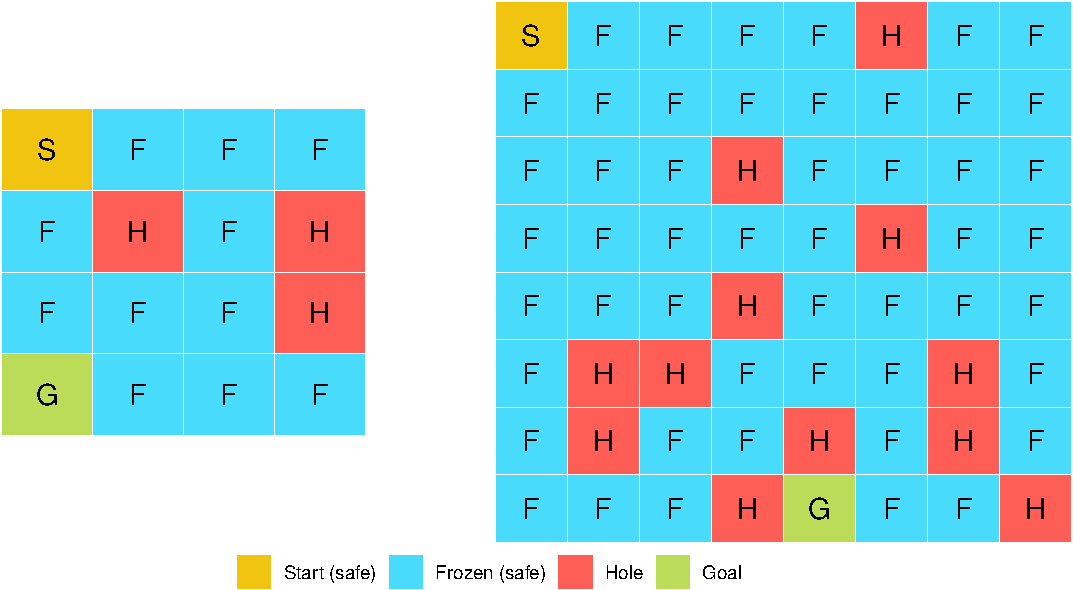
\includegraphics[width=0.7\linewidth]{project_files/figure-latex/environments-1} \end{center}

\section{Methodology}\label{methodology}

\section{Implementation}\label{implementation}

\subsection{Senseless Agent}\label{senseless-agent}

\subsection{Simple Agent}\label{simple-agent}

\subsection{Reinforcement Learning
Agent}\label{reinforcement-learning-agent}

\subsection{Environment Modifications}\label{environment-modifications}

In order to add additional flexibility and generic support to the
agents, slight changes were made to the \texttt{uofgsocsai.py} file, the
one containing the main \texttt{LochLomondEnv} environment class. The
changes below were approved as long as justification was provided. The
changes and justifications are as follows:

\begin{itemize}
\tightlist
\item
  Parameters \texttt{map\_name\_base}, \texttt{reward} and
  \texttt{path\_cost} where added to the \texttt{LochLomondEnv}
  constructor. The default values are \texttt{8x8-base}, \texttt{1.0}
  and \texttt{0} respectively. The default values do not alter the
  functionality from the original file provided.
\item
  Attributes \texttt{is\_stochastic}, \texttt{reward\_hole},
  \texttt{reward} and \texttt{path\_cost} were added to the class
\end{itemize}

The reason of the changes for the constructor was to add flexibility to
be able to test different scenarios without the need to modify the file
every time a different variant was analyzed. The attributes added to the
class in order to be able to access them via the object (e.g.
\texttt{env.path\_cost}) and create a Markov Decision Process out of it.
Even though a Markov Decision Process was out of the scope of this
project, an inhouse mapper from \texttt{Open\ AI\ Gym} environment to
Grid MDP with the only purpose of doing a sanity check between the final
U and policy from the Reinforcement Learning agent and the ones that a
\texttt{Policy\ Iteration} and \texttt{Value\ Iteration} algorithm would
provide.

Finally, the way to assign en environment grid was changed from
\texttt{MAPS\_BASE{[}map\_name\_base{]}} to
\texttt{copy.deepcopy(MAPS\_BASE){[}map\_name\_base{]}}, with the only
purpose of being able to instantiate the \texttt{LochLomondEnv} more
than once in a single run (e.g.
\texttt{python\ run\_rl.py\ 1,2,3,4,5,6,7}), which runs all the variants
in a single call.

There may be other better ways of accomplish the same without code
changes, but due to the current lack knowledge of Python programming,
time did not permit to find better ways for it.

\section{Evaluation}\label{evaluation}

Every agent produces different evaluation files that will be created
inside the \texttt{out} folder.

\section{Conclusions}\label{sec:con}

\newpage

\section{References}\label{references}

\newpage

\section{Appendices}\label{appendices}

\subsection{Appendix A: Title Here}\label{appendix-a-title-here}

\begin{figure}[h]

{\centering 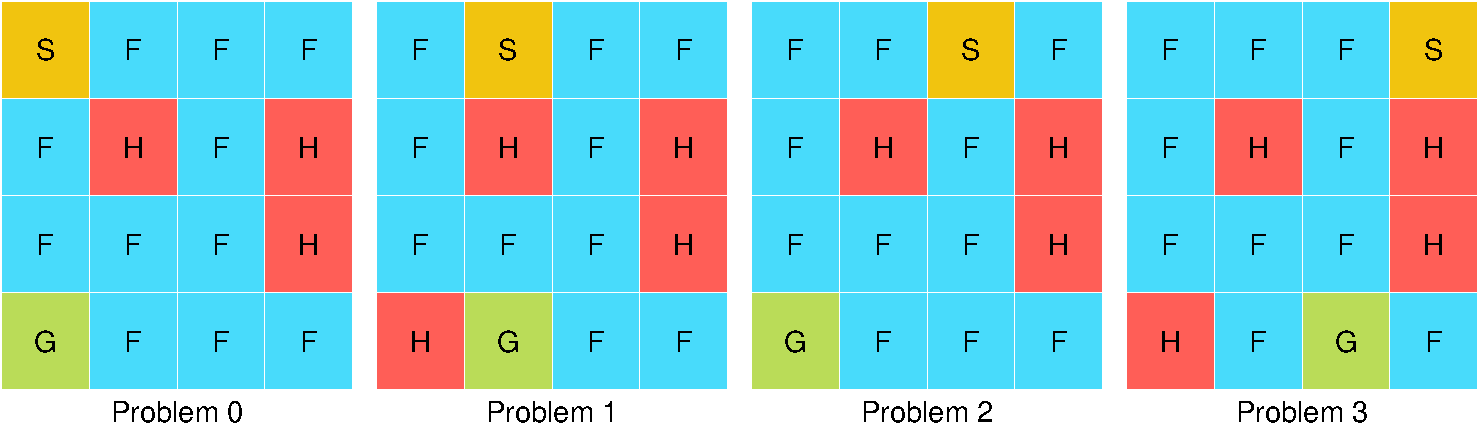
\includegraphics[width=0.9\linewidth]{project_files/figure-latex/unnamed-chunk-6-1} 

}

\caption{\label{fig:appendixa} My caption here}\label{fig:unnamed-chunk-6}
\end{figure}

\begin{figure}[h]

{\centering 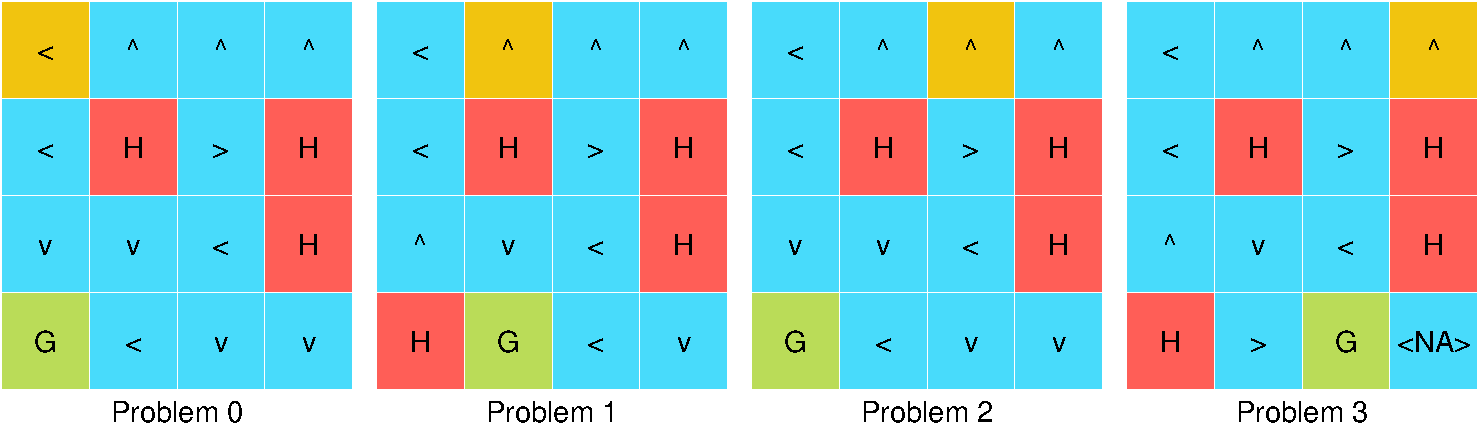
\includegraphics[width=0.9\linewidth]{project_files/figure-latex/unnamed-chunk-7-1} 

}

\caption{\label{fig:appendixa} My caption here}\label{fig:unnamed-chunk-7}
\end{figure}

\begin{figure}[h]

{\centering 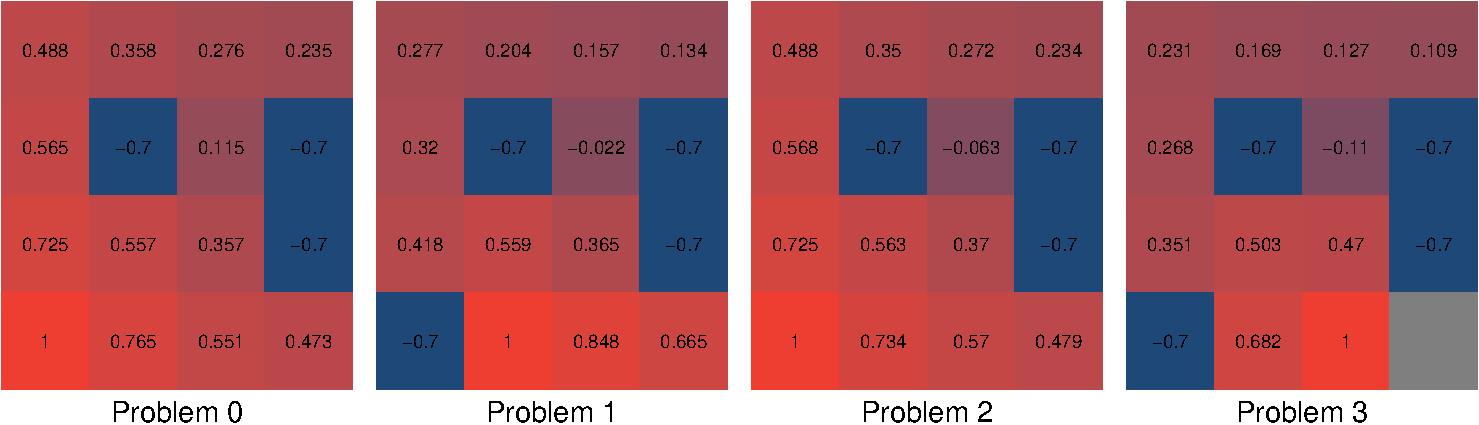
\includegraphics[width=0.9\linewidth]{project_files/figure-latex/unnamed-chunk-8-1} 

}

\caption{\label{fig:appendixa} My caption here}\label{fig:unnamed-chunk-8}
\end{figure}

\newpage

\subsection{Appendix B: Title Here}\label{appendix-b-title-here}

\begin{figure}[h]

{\centering 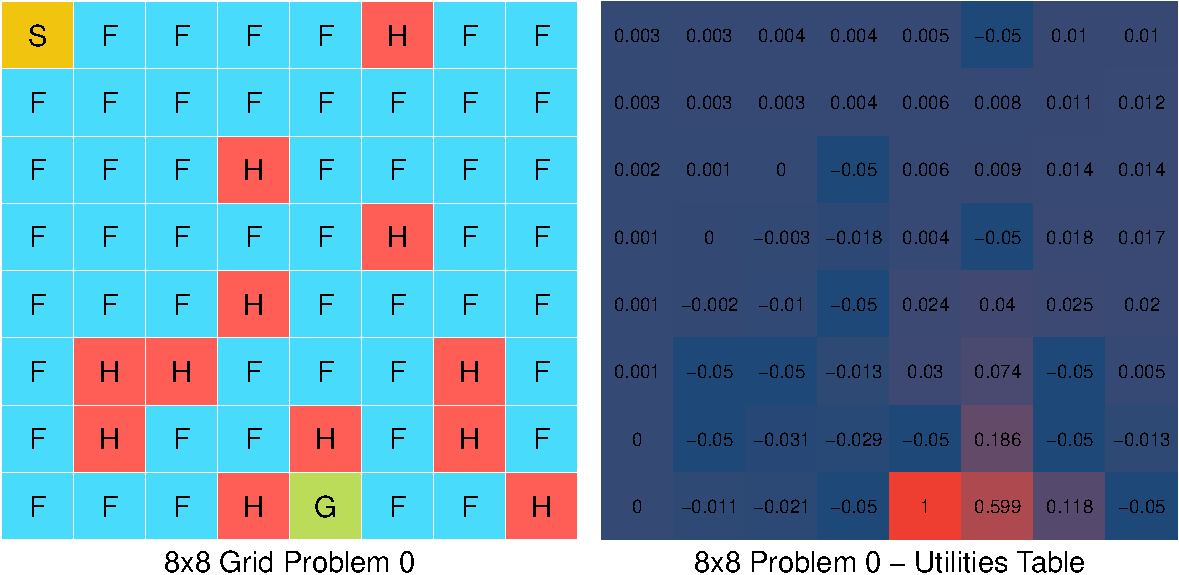
\includegraphics[width=0.85\linewidth]{project_files/figure-latex/lakes3-1} 

}

\caption{\label{fig:appendixa} My caption here}\label{fig:lakes31}
\end{figure}\begin{figure}[h]

{\centering 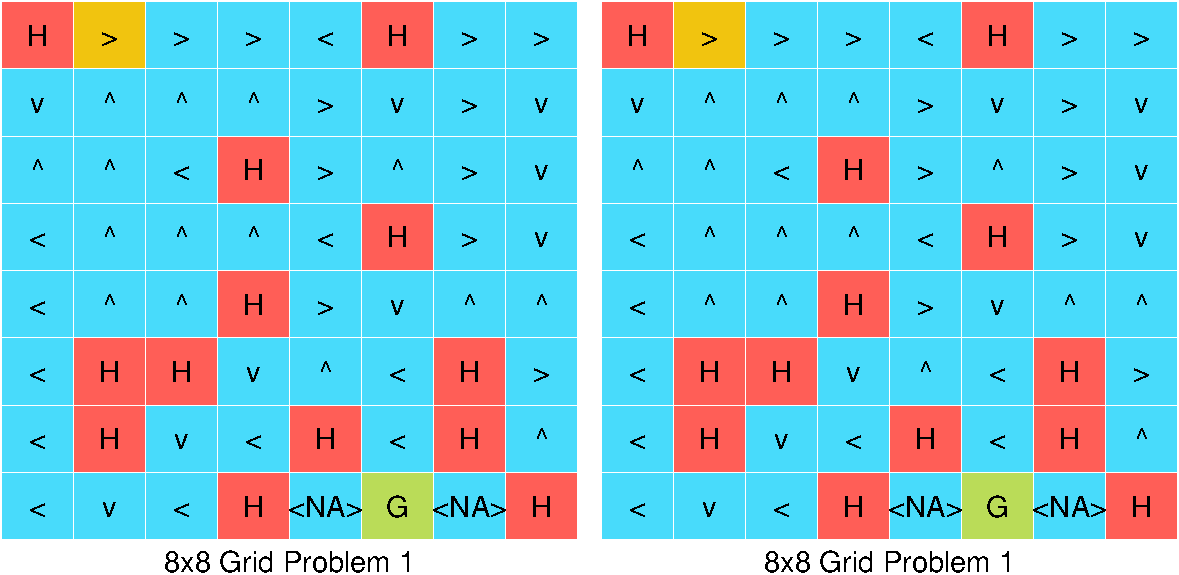
\includegraphics[width=0.85\linewidth]{project_files/figure-latex/lakes3-2} 

}

\caption{\label{fig:appendixa} My caption here}\label{fig:lakes32}
\end{figure}


\end{document}
